\documentclass[10pt, twocolumn, twoside]{article}

\usepackage[left=0.70cm, right=0.70cm, top=0.70cm, bottom=0.70cm]{geometry}
\usepackage{graphicx} %for importing graphics, see \begin{figure} below.
\usepackage{amssymb,amsmath} % add some standard packages for maths and symbols
\usepackage[colorlinks=true,linkcolor=blue]{hyperref} % turns all latex references into hyperlinks


\author{Jubayr Ahmed\\FY Physics Project}

\title{Discovering Dark Matter}

\date{\today}

\begin{document}

\maketitle %this uses the author, title, date information given in the preamble to make a title.

\begin{abstract}
Dark matter makes up the majority of what we are unable to observe in our universe, however it can be shown to exist by the differences between predictions and the observed results. For small objects there is almost equal parts mass and dark matter, but the dark matter growth is exponential, the more mass a celestial body has. The larger the mass, the greater the velocity up until a critical mass, after which point the velocity of a celestial object will gradually decrease to a constant.
\end{abstract}

\section{Introduction}
The discovery of dark matter as a component of our universe was a major discovery of the 20th century in physics. The first evidence for dark matter came from studying how fast stars rotate around the center of galaxies, the gravitational lens effect of light bending around large celestial bodies and more recently the discovery of CMBR (Cosmic Microwave Background Radiation) which places a limit over what we are able to detect of our universe. We can derive it from basic principles, starting with centripetal acceleration and the gravitational force between two masses.

\begin{equation}
a = \frac{v^2}{r}
\end{equation}

\begin{equation}
F = \frac{G M m}{r^2} = ma
\end{equation}

\begin{equation}
\frac{G M m}{r^2}=\frac{m v^2}{r}
\end{equation}

\begin{equation}
\therefore v = \sqrt{\frac{GM}{r}}
\end{equation}

Now imagine that instead of circling an object, the small mass, m, is circling in a uniform cloud of gas with density $\rho$. The mass, M, that goes into the gravitational force equation in this case is only the mass in the sphere contained within the orbit of the small mass. We’ll call this M$_c$.

\begin{equation}
M_c(r) = \frac{4}{3}\pi r^3\rho
\end{equation}

\begin{equation}
\therefore v = \sqrt{\frac{4G\pi r^3\rho}{3r}} = r\sqrt{\frac{4}{3}G\pi\rho} 
\end{equation}

What has been shown here is that the velocity is directly related to the radius. However, we can continue further and show that dark matter is related to the mass density and radius. We now introduce two constants: $\rho_0$ which controls the overall amount of dark matter and $r_c$ which is known as the critical radius and this controls how quickly density decreases as a function of the radius.

\footnote{G = 4.3x10^-^6 kpc/M, \rho_0 = 100x10^6M/(kpc)^3, r_c = 1.87 kpc}

\begin{equation}
\rho(r) = \frac{\rho_0}{1+\frac{r}{r_c^2}}
\end{equation}

\begin{equation}
M_c^D^M = \int_0^r \frac{\rho_04\pi R^2 d R}{1+(\frac{R}{r_c})^2}
\end{equation}

\begin{equation}
\therefore M_c^D^M = 4\pi\rho_0\int_0^r \frac{R^2 d R}{1+(\frac{R}{r_c})^2}
\end{equation}

\begin{equation}
\therefore M_c^D^M = 4\pi\rho_0r_c^2(r-r_c\arctan(\frac{r}{r_c})) 
\end{equation}

\section{Method}
We analysed one set of galaxy data that has been provided containing mass, radius and velocity of fifty celestial bodies. After we compare that to another set of galaxy data. We worked out the predicted velocity, the mass of dark matter and the combined total of the mass and dark matter per celestial body using equations in repl.it with a python3 extension. We then plotted graphs.

\section{Plots and Analysis}

\newpage

\begin{figure}[ht]
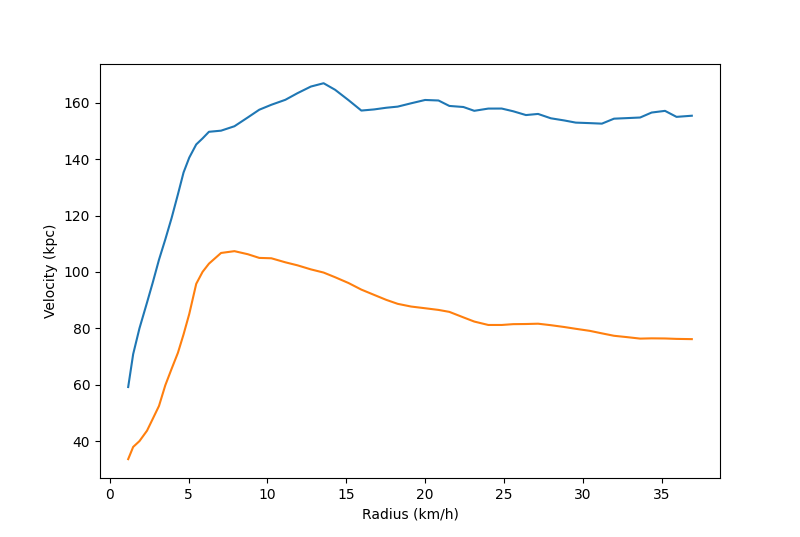
\includegraphics[width=\columnwidth]{graph1.png}
\caption[width=\columnwidth]{Velocity plotted against Radius of Galaxy 1}
\end{figure}

What we can see here is that for our designated galaxy, the predicted velocity of celestial bodies in that galaxy is significantly lower than what is observed and the velocity plateaus past a certain radius (around 7kpc). this is the critical radius for that galaxy. This would suggest that there is an unknown variable surrounding the celestial bodies which is affecting the measurements and making the velocity higher than what would be predicted.

\begin{figure}[ht]
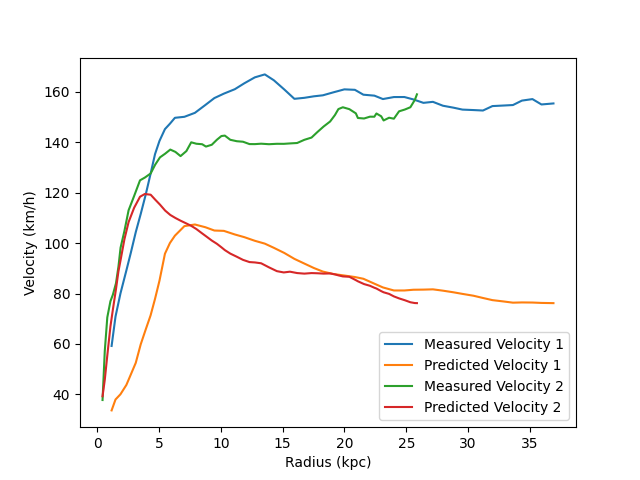
\includegraphics[width=\columnwidth]{graph6.png}
\caption[width=\columnwidth]{Velocity plotted against Radius of Galaxies 1 and 2}
\end{figure}

When comparing to our second galaxy we see that critical radius at which the velocity plateaus is much shorter (around 5kpc). The velocity is lower in comparison to the first galaxy, however the predicted velocity of the second galaxy is much closer to the measured velocity than that of the first galaxy. This shows that the unknown variable has different quantities that vary from galaxy to galaxy.

\newpage

\begin{figure}[ht]
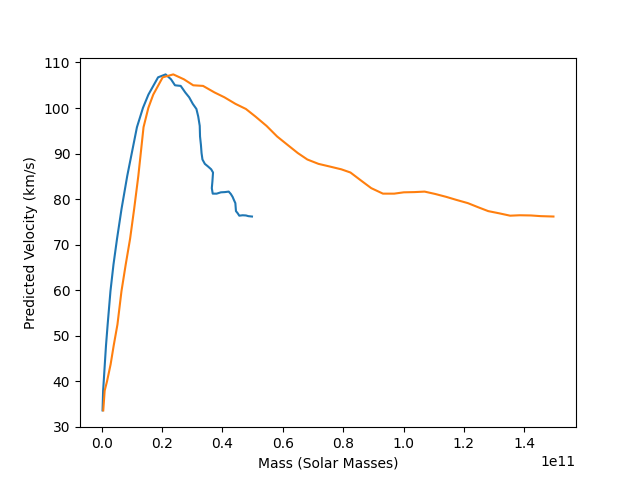
\includegraphics[width=\columnwidth]{graph2.png}
\caption[width=\columnwidth]{Predicted Velocity plotted against Mass of Galaxy 1}
\end{figure}

From this graph we can see that the velocity of measured mass and the calculated dark matter are almost equal, up until the 0.25 solar mass plateau point, but beyond this point the Dark Matter drops off at a much slower rate and keeps going for much larger solar masses. The velocity of a mass past a critical radius appears to slow down gradually to a constant velocity around 75km/h.

\begin{figure}[ht]
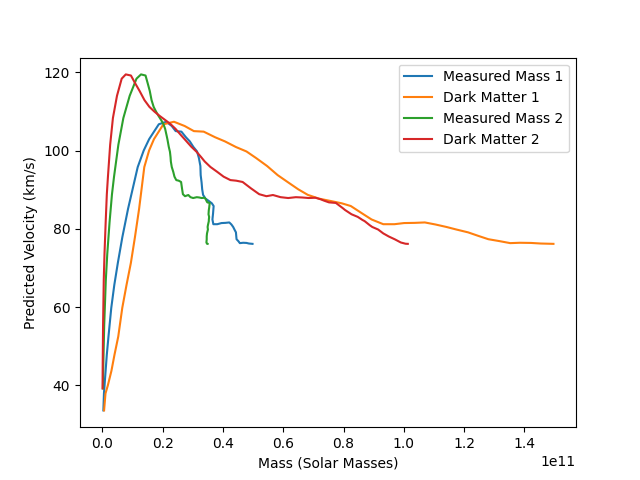
\includegraphics[width=\columnwidth]{graph7.png}
\caption[width=\columnwidth]{Predicted Velocity plotted against Mass of Galaxies 1 and 2}
\end{figure}

Comparing the two galaxies we can see that the mass and dark matter contained in galaxy 2 is a lot larger and the velocity increases more drastically than galaxy 1, but plateaus at a much shorter mass (0.14 solar masses). This reinforces the fact that the amount of dark matter varies from galaxy to galaxy but the relationship between mass and dark matter is almost linear until the plateau point. Galaxy 2 also has a lower constant velocity after the celestial body goes past the critical mass, around 70km/h

\newpage

\begin{figure}[ht]
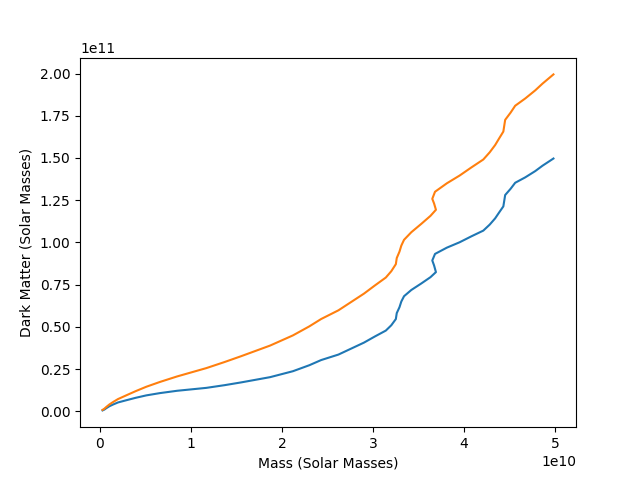
\includegraphics[width=\columnwidth]{graph3.png}
\caption[width=\columnwidth]{Dark Matter plotted against Mass}
\end{figure}

Reinforcing the point above, the relationship between dark matter is linear, but when we plot the total mass against dark matter we see that dark matter increases much faster the greater the mass. The gradient for the mass is 1/12 whereas for the total mass, the gradient increases to 1/6. this would mean that there are almost equal parts dark matter to matter for celestial bodies of smaller mass but this exponentially increases the larger the mass of the object.

\begin{figure}[ht]
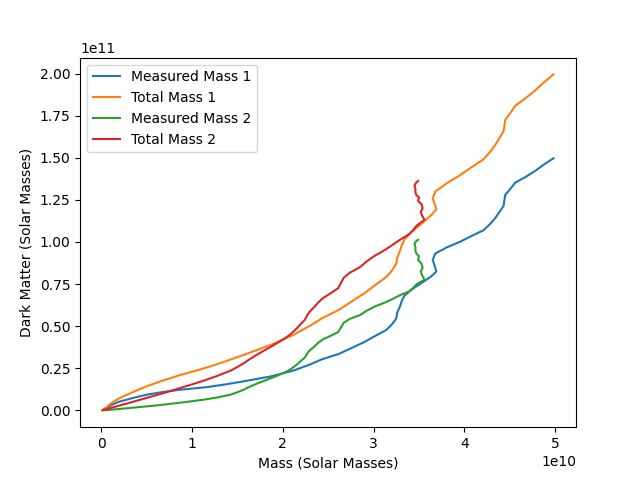
\includegraphics[width=\columnwidth]{graph8.png}
\caption[width=\columnwidth]{Dark Matter plotted against Mass of Galaxies 1 and 2}
\end{figure}

Here we do not see much of a difference between the two galaxies. They follow the same linear pattern, which means that dark matter is consistently. if we drew a line of best fit representing all the data sets, the gradient would be around 1/6 for both galaxies until around 3.5 solar masses where the graph starts to increase exponentially.

\newpage

\section{Conclusions}

For small objects there is almost equal parts mass and dark matter, but the dark matter growth is exponential the more mass a celestial body has. The larger the mass, the greater the velocity up until a critical mass, after which point the velocity of a celestial object will gradually decrease to a constant. No two galaxies are the same as they all contain celestial bodies of varying masses and velocities, but they follow these same general rules.

\section{Reflection}
With limited python knowledge and less so of git, this was more challenging and took more time to comprehend the data and questions. As a result it took far more time to do some of the tasks and the later tasks such as implementing trendlines and equations were almost to difficult to implement properly. Not to mention that quarantine has not helped with my understanding or concentration when it came to some of these new ideas. When it came to writing the report with latex, it also took a lot longer to do as it behaves more like a programming software/editor rather than say something like a word processor.

\end{document}